\documentclass{article} % For LaTeX2e
\usepackage{nips14submit_e,times}
\usepackage{hyperref}
\usepackage{url}
\usepackage[pdftex]{graphicx}	
\usepackage{float}
\usepackage[caption = false]{subfig}
%\documentstyle[nips14submit_09,times,art10]{article} % For LaTeX 2.09

\title{Visualization of Community Structures in Scientific Networks}

\author{
Yuan Huang \\
Department of Physics\\
University of Massachusetts, Amherst\\
Amherst, MA, 01002 \\
\texttt{yuanh@physics.umass.edu} \\
}

% The \author macro works with any number of authors. There are two commands
% used to separate the names and addresses of multiple authors: \And and \AND.
%
% Using \And between authors leaves it to \LaTeX{} to determine where to break
% the lines. Using \AND forces a linebreak at that point. So, if \LaTeX{}
% puts 3 of 4 authors names on the first line, and the last on the second
% line, try using \AND instead of \And before the third author name.

\newcommand{\fix}{\marginpar{FIX}}
\newcommand{\new}{\marginpar{NEW}}
\nipsfinalcopy % Uncomment for camera-ready version

\begin{document}

\maketitle

\section{Introduction}
\label{intro}

Detecting community structure is an important task in the field of complex networks. Community structure refers to that the vertices in networks tend to cluster into different groups with a large number of within-group edges and a small number of edges between groups. In this paper, we focus on the community structure in the citation networks of academic articles. The analysis of the underlying community structure in citation networks provides numerous benefits for the development of the research field, including building a foundation for future research through the acknowledgement of past research activities; identifying gaps in research for researchers and students; improving the integration between theory and practice, and so on~\cite{phys_rev, OLED, learning_analytics, sustain}. On the other hand, finding clusters in network-structured data is a fundamental problem that has many applications in social networks and other related fields. 

As I start this project, I wish to use various network visualization to answer the following questions: 1) How do different subfields of physics evolve in time? Which subfields are fast growing in recent years? 2) Who are the physicists with most impact in a specified field of physics? How are the top physicists interacting with each other (through citation and collaboration)? 3) What are the top institutions for a specified field? How are the institutions collaborating with each other? So far, the project includes the first two questions regarding the subfield analysis and top physicists in a specified field. Hopefully the intitutions analysis can be realized in the future.


%%%%Add results

\section{Related Works}
\label{related}
The analysis of citation and co-authorship network has been performed for many research fields, such as organic LED~\cite{OLED}, learning analysis~\cite{learning_analytics}, sustainable science~\cite{sustain}, and so on. The study of the community structure has been attracting more and more interest in the field of scientific network study. In recent years, a growing number of clustering algorithms for categorical data have been proposed to study the community structure of the scientific networks~\cite{Newman_divisive, bottom_up, new_method, Newman_evaluation,  method_review, Newman_algorithm}. 

In 2008, Leicht and Newman~\cite{Newman_divisive} proposed a general divisive hierarchical clustering algorithm for network. The method try to maximize the modularity of the graph using the eigenvalues and eigenvectors of the modularity matrix. By iteratively divide each group into subgroups according to the leading eigenvectors of the modularity matrix, the algorithm can achieve the clustering that maximize the global modularity. 

At the same year, Blondel et. al.~\cite{bottom_up} proposed a highly efficient agglomerative clustering algorithm. Here each network node is initially assigned to a unique community. Then, the algorithm iteratively groups the pair of nodes that maximizes the increase of the global modularity into the same community, until a maximal modularity is achieved. This algorithm is computationally more efficient than the previous divisive approach but has the disadvantage of requiring more memory. 

In 2010, Chen and Redner~\cite{phys_rev} investigated the community structure of physics subfields in the citation network of well-cited Physical Review Publications (with more than 100 citations). In their paper, they applied the divisive hierarchical algorithm based on modularity maximization~\cite{Newman_divisive} to identify community within networks and performed analysis on the major communities. They also examined communities decade by decade and found a small number of significant links between communities that are widely separated in time. 

In 2011, Zhao and Zhang~\cite{new_method} proposed a new clustering method for detecting community structures. In this method, individuals and their relationships are denoted by weighted graphs, then the graph density gives a better quantity depict of whole correlation among individuals in a community, so that a reasonable clustering output can be presented. By constructing a non-binary hierarchical tree of clusters, this method has two important features: one is that the hierarchical tree is much smaller that clearly highlights meaningful clusters; the other one is the clusters can overlap with each other which does reflect the complexity of our real world.

\section{Data Sets}
\label{data}

The data set has been requested from the American Physics Society website and contains over 450,000 articles from Physical Review Letters, Physical Review, and Reviews of Modern Physics dating from 1893 to 2015. The data sets have two parts:
(1) citing article pairs, which consists of pairs of APS articles that cite each other in format "10.1103/PhysRevSeriesI.11.215, 10.1103/PhysRevSeriesI.1.1"(first string is the doi of the citing article, while the second string is the doi of the cited article); (2) article metadata which consists of the basic metadata of all APS journal articles including doi, title, journal, date, volume, page, author, affiliations, and so on (each article is stored in individual json files).

In this project, we will focus on all the articles published in Physical Review Letter, Review of Modern Physics, and Physical Review X from 2007 to 2015, and perform clustering algorithm on the citation network of these articles. To get this subset of citation network, we load all the article metadata and citation data into a mongodb database, and use the journal and date features in the metadata to filter the citation data. This results in a network of 27695 articles and 91346 citation links between them.

The clustering analysis and visualizations of the citation network and community structures can help the users to learn about the research history in physics and identify interesting fields. After identifying a subfield which is potentially interesting, the visualizations of the community networks can help the users to find out the top physicists that are working on the selected field, papers with the most impacts in the field, and see the trend of each field in physics.

\section{Exploratory Analysis}

In this project, we apply a hierarchical clustering algorithm based on modularity maximization to cluster the network of 27695 articles and 91346 citation links. The first step is to use pymongo to load the mongo database in python. Then we apply the clustering algorithm for the citation network data.

Modularity maximization is a bottom-up hierarchical clustering algorithm which repeatedly merges two clusters into one in order to optimize the modularity of the clustering. This algorithm works as follows: Starting from a state where each node is in its unique community, we repeatly join pairs of communities into one, until we reach the maximal modularity. I implement this algorithm from scratch using python and apply this clustering algorithm on the citation network. The modularity function peaks at $Q = 0.762$, when the number of cluster is 500, shown in Fig~\ref{fig:modularity_whole_a}. This value is rather high in real world network data, indicating a strong community structure in our citation network. 
As we perform analysis on the clustering result, one observation is that the size of clusters features a power-law distribution, where the largest cluster has nearly 5000 articles, while the majority of clusters are rather small with less than 1000 articles, shown in Fig~\ref{fig:modularity_whole_b}. In this project, we decide to focus on the large clusters with more than 1000 articles (there are 13 large clusters in total) since they are more representative as different fields in physics. 

\begin{figure}[h]
  	\centering
	\vspace{-20pt}
	\subfloat[][Modularity function.]{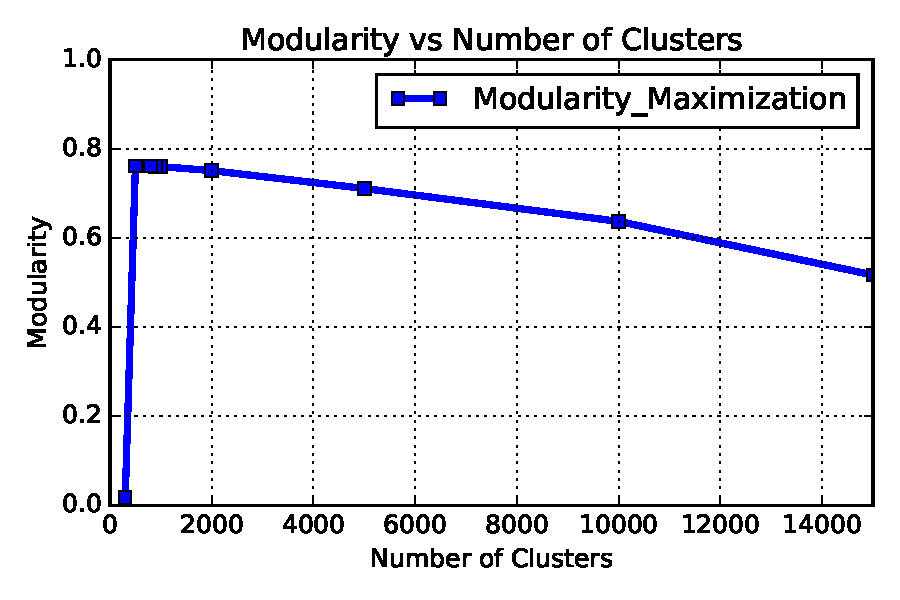
\includegraphics[width = 3in]{./Figures/Modularity_Maximization_modularity_score_whole.pdf}\label{fig:modularity_whole_a}}
  	\subfloat[][Cluster size distribution.]{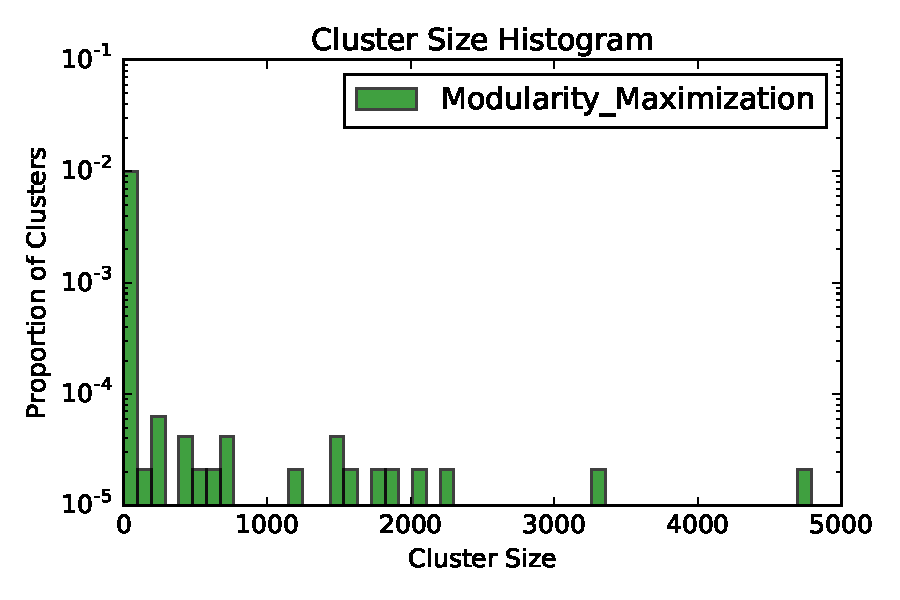
\includegraphics[width = 3in]{./Figures/Modularity_Maximization_cluster_size_whole.pdf}\label{fig:modularity_whole_b}}
 	\caption{The modularity function, and the cluster size distribution function in the simulation with the modularity maximization algorithm on the citation network.}
 	\vspace{-10pt}
  \label{fig:modularity_whole}
\end{figure}

With the obtained clustering result, we can perform different analysis on the dataset. First, we query the database using pymongo library to obtain the papers with high citation numbers in each cluster. As we look at those papers with high impact, we summarize the topic in each cluster and use it as the cluster's name. Then, we extract the number of articles published over time for each cluster to study the trend in physics research. Another useful analysis is the authors with the most publications in each field of physics. From this analysis, we can identify the physicists with high impact in different fields. All the results from these analysis are dumped into json files for visualizations.

\section{Implementations of Visualizations}

The implementation of the visualizations are based on D3, NVD3, bootstrap, jqurey libraries. The landing page and layout design are based on start bootstrap templates. The visualizations on the webpage include two parts: the visualizations for articles, and physicists.

\subsection{Articles}
The network of articles is visualized using D3 force-layout bubble charts(Fig~\ref{fig:cluster_whole}). The size of bubbles represents the number of articles in each community, while the width of links represents the number of citations between two communities. Clicking on each bubble in the first and second charts will trigger the chart to its right to show the corresponding structures inside the clicked cluster. In the right most chart with network of each individual articles, clicking on each node will open a new tab in your browser and go to the APS webpage of the selected article.

\begin{figure}[h]
  	\centering
  	\subfloat[][]{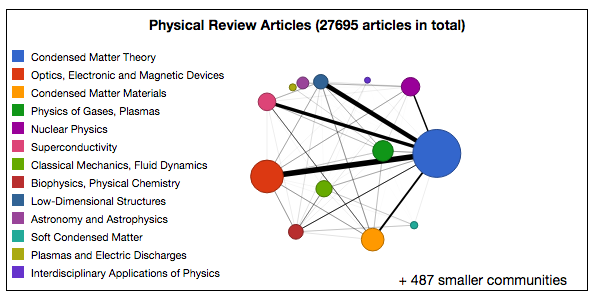
\includegraphics[width = 3in]{./Figures/visualization_whole.png}}
  	\subfloat[][]{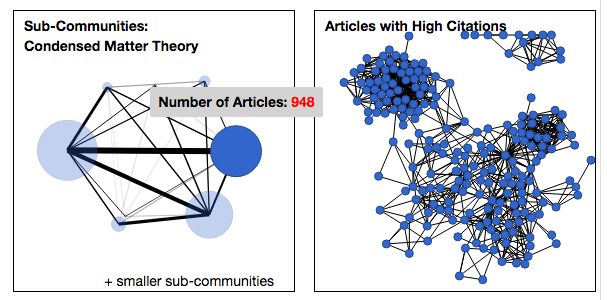
\includegraphics[width = 3.05in]{./Figures/visualization_cm.png}}
 	\caption{Visualizations of the network of articles.}
 	\vspace{-10pt}
  \label{fig:cluster_whole}
\end{figure}

The evolution of communities over time is visualized using stacked area charts implemented with NVD3 library(Fig~\ref{fig:theme_river}). The visualizations support selections, probing, and changing layout. Select one area in the left chart will trigger the right chart to show the corresponding sub-fields in the select field. Selecting in either the left most cluster bubble chart or the left stacked area chart will simultaneously trigger all the rest charts to respond.

\begin{figure}[h]
  	\centering
    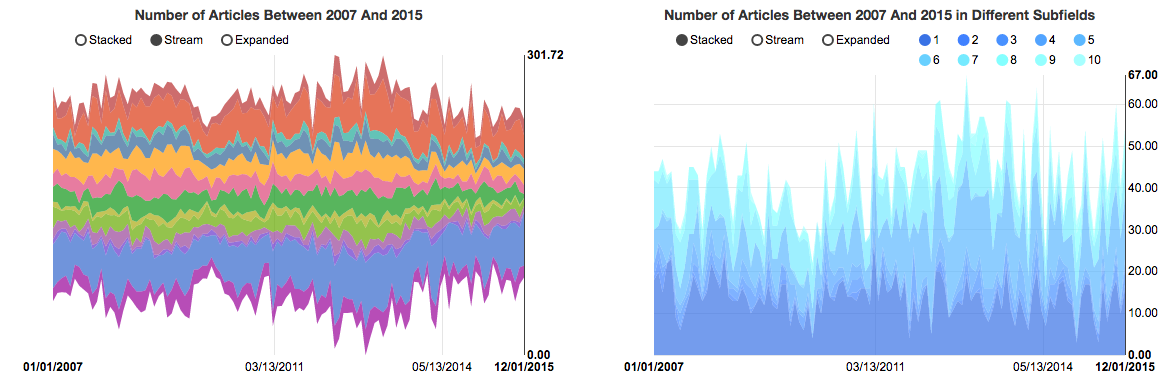
\includegraphics[width = 5in]{./Figures/theme_river.png}
 	\caption{Visualizations of the evolution of different fields in time.}
 	\vspace{-10pt}
  \label{fig:theme_river}
\end{figure}
 
\subsection{Physicists}
The physicists in different fields is visualized using D3 force-layout bubble charts(Fig~\ref{fig:author_whole}). The left chart is the same with the first chart in the network of articles. The right one shows the physicists from different fields, represented by bubbles with color denoting the field, and size denoting the number of publications. The typical number of publications in different fields vary dramatically, therefore I normalize the size according to the largest node in each cluster. One interesting observation is that the authors in nuclear physics and astrophysics tend to publish much more papers than other fields. Clicking on a bubble in the left chart will highlight the selected field in the right chart. Clicking on each individual node in the right bubble chart will open a new tab in your browser and start a Google search for the selected physicist.

\begin{figure}[h]
  	\centering
    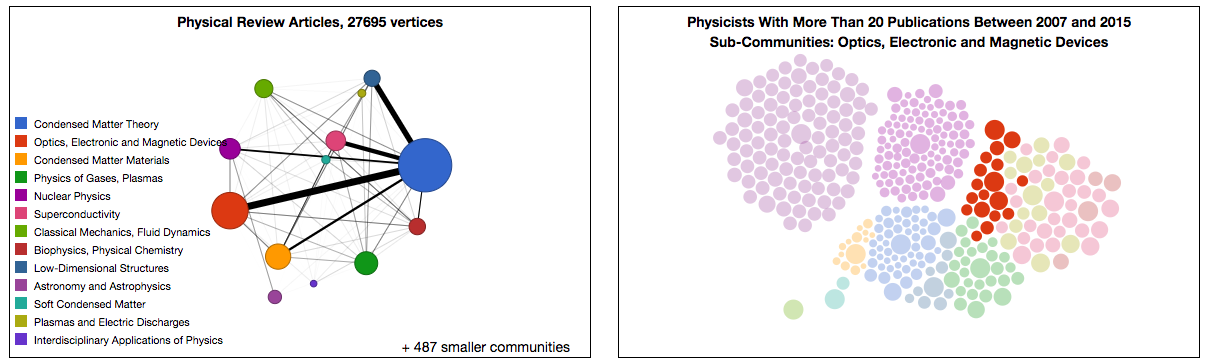
\includegraphics[width = 5in]{./Figures/author_whole.png}
 	\caption{Visualizations of the physicists in different fields.}
 	\vspace{-10pt}
  \label{fig:author_whole}
\end{figure}

\section{Links}
The link to the webpage is \url{http://www-edlab.cs.umass.edu/~yuanh/590v/project/pages/index.html}.

The whole dataset can be requested at \url{https://journals.aps.org/datasets}.

\section{Acknowledgements}
I want to thank the \href{https://journals.aps.org/}{American Physical Society} for offering the dataset for this project. Image credits to \href{https://wallpapersafari.com/w/fKpsS1}{Martin Driver}, \href{http://img15.deviantart.net/b424/i/2013/157/b/f/the_hitchhiker_s_guide_to_the_galaxy_wallpaper_by_lucaszanella-d6821pm.png}{deviantart.net}., and \href{https://society6.com/product/dont-panic-9mv_print#s6-1258355p4a1v45}{society6.com}. The webpage template is adapted from \href{https://startbootstrap.com/}{Start Bootstrap}.

\small{
\begin{thebibliography}{9}
\bibitem{phys_rev}
P. Chen, S. Redner. \textit{Community structure of the physical review citation network}, Journal of Informetrics, {\bf 4} (2010) 278-290.

\bibitem{OLED}
Y. Kajikawa, Y. Takeda. \textit{Citation network analysis of organic LEDs}, Technological Forecasting and Social Change, {\bf 76} (2009) 1115-1123.

\bibitem{learning_analytics}
S. Dawson, D. Gasevic, G. Siemens, S. Joksimovic. \textit{Current State and Future Trends: A Citation Network Analysis of the Learning Analytics Field}, In Proceedings of the Fourth International Conference on Learning Analytics And Knowledge (LAK 2014). ACM, New York, NY, USA, 231-240.

\bibitem{sustain}
Y. Kajikawa, J. Ohno, Y. Takeda, K. Matsushima, H. Komiyama. \textit{Creating an academic landscape of sustainability science: an analysis of the citation network}, Sustain Science, (2007) {\bf 2}:221-231.

\bibitem{Newman_divisive} E. A. Leicht, and M. E. J. Newman. \textit{Community structure in directed networks}, Physical Review Letters, (2008) {\bf 100}, 118703.

\bibitem{bottom_up} V. D. Blondel, J. L. Guillaume, R. Lambiotte, and E. Lefebvre, E. (2008). \textit{Fast unfolding of communites in large networks}, Journal of Statistical Mechanics: Theory and Experiment, P1008, 1742–5468.

\bibitem{new_method}
P. Zhao, and C. Zhang. \textit{A new clustering method and its application in social networks}, Pattern Recognition Letters {\bf 32} (2011) 2109-2118.

\bibitem{Newman_evaluation}
M. E. J. Newman, and M. Girvan. \textit{Finding and evaluating community structure in networks}, Phys. Rev. E {\bf 69}, 026113 (2004).

\bibitem{method_review}
L. Danon, A. Diaz-Guilera, J. Duch, and A. Arenas. \textit{Comparing community structure identification}, J. Stat. Mech. (2005) P09008.

\bibitem{Newman_algorithm}
M. E. J. Newman. \textit{Fast algorithm for detecting community structure in networks}, Phys. Rev. E {\bf 69}, 066133 (2004).

\end{thebibliography}
}

\end{document}
